%#BIBTEX pbibtex star_a10
%%%%%%%%%%%%%%%%%%%%%%%%%%%%%%%%%%%%%%%%%%%%%%%%%%%%%%%%%%%%%%%%%%%%%%%%%%%%%
%集録提出用のサンプルファイルです。
%このファイルを参考にして集録を作成してください。
%%%%%%%%%%%%%%%%%%%%%%%%%%%%%%%%%%%%%%%%%%%%%%%%%%%%%%%%%%%%%%%%%%%%%%%%%%%%%
%%%%%%%%%%%%%%%%%%%%%%%%%%%%%%%%%%%%%%%%%%%%%%%%%%%%%%%%%%%%%%%%%%%%%%%%%%%%%
\documentclass[a4paper,10pt,oneside,twocolumn,notitlepage,final]{jarticle}
\usepackage{ss18_UTF-8}
%%%%%%%%%%%%%%%%%%%%%%%%%%%%%%%%%%%%%%%%%%%%%%%%%%%%%%%%%%%%%%%%%%%%%%%%%%%%%
%%ss18.styファイルはtexファイルと同じディレクトリに置いてください。
%%ヘッダ、フッターなどの全体のレイアウトは変更しないでください。
%%ここより上は変更しないでください。
%%%%%%%%%%%%%%%%%%%%%%%%%%%%%%%%%%%%%%%%%%%%%%%%%%%%%%%%%%%%%%%%%%%%%%%%%%%%%
%%使いたいパッケージがある場合は以下に書いてください。
\usepackage[dvipdfmx]{graphicx,color}
\usepackage{caption}
\usepackage[font=small]{subcaption}
%\captionsetup{compatibility=false}
\captionsetup[figure]{format=plain, labelformat=simple, labelsep=colon, font=small}
\usepackage{here}
\usepackage{chngcntr}

\renewcommand{\refname}{参考文献}


%%%%%%%%%%%%%%%%%%%%%%%
\makeatletter
\renewenvironment{thebibliography}[1]
{\section*{\refname\@mkboth{\refname}{\refname}}%
  \list{\@biblabel{\@arabic\c@enumiv}}%
       {\settowidth\labelwidth{\@biblabel{#1}}%
         \leftmargin\labelwidth
         \advance\leftmargin\labelsep
         \setlength\itemsep{-0.0zh}%←ここの数値を調整(行間のつまり具合)
         \setlength\baselineskip{10pt}%←ここの数値を調整(追加)(文字の大きさ)
         \@openbib@code
         \usecounter{enumiv}%
         \let\p@enumiv\@empty
         \renewcommand\theenumiv{\@arabic\c@enumiv}}%
       \sloppy
       \clubpenalty4000
       \@clubpenalty\clubpenalty
       \widowpenalty4000%
       \sfcode`\.\@m}
{\def\@noitemerr
  {\@latex@warning{Empty `thebibliography' environment}}%
  \endlist}
\makeatother
%%%%%%%%%%%%%%%%%%%%%%%



\def\aj{AJ}%
         % Astronomical Journal
\def\actaa{Acta Astron.}%
         % Acta Astronomica
\def\araa{ARA\&A}%
         % Annual Review of Astron and Astrophys
\def\apj{ApJ}%
         % Astrophysical Journal
\def\apjl{ApJ}%
         % Astrophysical Journal, Letters
\def\apjs{ApJS}%
         % Astrophysical Journal, Supplement
\def\ao{Appl.~Opt.}%
         % Applied Optics
\def\apss{Ap\&SS}%
         % Astrophysics and Space Science
\def\aap{A\&A}%
         % Astronomy and Astrophysics
\def\aapr{A\&A~Rev.}%
         % Astronomy and Astrophysics Reviews
\def\aaps{A\&AS}%
         % Astronomy and Astrophysics, Supplement
\def\azh{AZh}%
         % Astronomicheskii Zhurnal
\def\baas{BAAS}%
         % Bulletin of the AAS
\def\bac{Bull. astr. Inst. Czechosl.}%
         % Bulletin of the Astronomical Institutes of Czechoslovakia
\def\caa{Chinese Astron. Astrophys.}%
         % Chinese Astronomy and Astrophysics
\def\cjaa{Chinese J. Astron. Astrophys.}%
         % Chinese Journal of Astronomy and Astrophysics
\def\icarus{Icarus}%
         % Icarus
\def\jcap{J. Cosmology Astropart. Phys.}%
         % Journal of Cosmology and Astroparticle Physics
\def\jrasc{JRASC}%
         % Journal of the RAS of Canada
\def\mnras{MNRAS}%
         % Monthly Notices of the RAS
\def\memras{MmRAS}%
         % Memoirs of the RAS
\def\na{New A}%
         % New Astronomy
\def\nar{New A Rev.}%
         % New Astronomy Review
\def\pasa{PASA}%
         % Publications of the Astron. Soc. of Australia
\def\pra{Phys.~Rev.~A}%
         % Physical Review A: General Physics
\def\prb{Phys.~Rev.~B}%
         % Physical Review B: Solid State
\def\prc{Phys.~Rev.~C}%
         % Physical Review C
\def\prd{Phys.~Rev.~D}%
         % Physical Review D
\def\pre{Phys.~Rev.~E}%
         % Physical Review E
\def\prl{Phys.~Rev.~Lett.}%
         % Physical Review Letters
\def\pasp{PASP}%
         % Publications of the ASP
\def\pasj{PASJ}%
         % Publications of the ASJ
\def\qjras{QJRAS}%
         % Quarterly Journal of the RAS
\def\rmxaa{Rev. Mexicana Astron. Astrofis.}%
         % Revista Mexicana de Astronomia y Astrofisica
\def\skytel{S\&T}%
         % Sky and Telescope
\def\solphys{Sol.~Phys.}%
         % Solar Physics
\def\sovast{Soviet~Ast.}%
         % Soviet Astronomy
\def\ssr{Space~Sci.~Rev.}%
         % Space Science Reviews
\def\zap{ZAp}%
         % Zeitschrift fuer Astrophysik
\def\nat{Nature}%
         % Nature
\def\iaucirc{IAU~Circ.}%
         % IAU Cirulars
\def\aplett{Astrophys.~Lett.}%
         % Astrophysics Letters
\def\apspr{Astrophys.~Space~Phys.~Res.}%
         % Astrophysics Space Physics Research
\def\bain{Bull.~Astron.~Inst.~Netherlands}%
         % Bulletin Astronomical Institute of the Netherlands
\def\fcp{Fund.~Cosmic~Phys.}%
         % Fundamental Cosmic Physics
\def\gca{Geochim.~Cosmochim.~Acta}%
         % Geochimica Cosmochimica Acta
\def\grl{Geophys.~Res.~Lett.}%
         % Geophysics Research Letters
\def\jcp{J.~Chem.~Phys.}%
         % Journal of Chemical Physics
\def\jgr{J.~Geophys.~Res.}%
         % Journal of Geophysics Research
\def\jqsrt{J.~Quant.~Spec.~Radiat.~Transf.}%
         % Journal of Quantitiative Spectroscopy and Radiative Trasfer
\def\memsai{Mem.~Soc.~Astron.~Italiana}%
         % Mem. Societa Astronomica Italiana
\def\nphysa{Nucl.~Phys.~A}%
         % Nuclear Physics A
\def\physrep{Phys.~Rep.}%
         % Physics Reports
\def\physscr{Phys.~Scr}%
         % Physica Scripta
\def\planss{Planet.~Space~Sci.}%
         % Planetary Space Science
\def\procspie{Proc.~SPIE}%
         % Proceedings of the SPIE



%%%%%%%%%%%%%%%%%%%%%%%%%%%%%%%%%%%%%%%%%%%%%%%%%%%%%%%%%%%%%%%%%%%%%%%%%%%%%
%%名前、所属、タイトルは以下に記入してください。
%%所属は以下のように()内にお願いします。
\author{磯谷 和秀 (名古屋大学大学院 理学研究科)}
\title{巨大衝突ステージにおける惑星-微惑星間の力学的摩擦と\\微惑星間の衝突・破壊の関係}
%%%%%%%%%%%%%%%%%%%%%%%%%%%%%%%%%%%%%%%%%%%%%%%%%%%%%%%%%%%%%%%%%%%%%%%%%%%%%


\begin{document}


%%概要は\abst内に記入してください。
%%\maketitleは必要ありません。
%%以下の\abst{}に概要を記入することにより
%%タイトル、名前、日付、概要が一括して出力されます。
\abst{
太陽系の地球型惑星は、最終段階で火星サイズの原始惑星同士が衝突合体を繰り返し形成されたと考えられており、この進化段階は巨大衝突ステージと呼ばれる。
%巨大衝突ステージを模擬し原始惑星の$N$体計算を行うと、合体成長を繰り返し数億年程度で現在の太陽系の地球型惑星のようないくつかの地球質量の惑星が形成される。
%しかし、原始惑星同士が軌道交差を起こすほど軌道が歪んだ状態で衝突合体が起きるため、最終的に形成される地球型惑星の離心率($\sim0.1$)は、現在の太陽系の地球型惑星の離心率($\sim0.01$)を説明できない。
%これに関する現在の惑星形成論の理解では、地球型惑星が形成された後に残存する微惑星との力学的摩擦によって地球型惑星の離心率が下げられるという説が有力である。
微惑星から原始惑星、原始惑星から惑星までの合体成長を$N$体計算で模擬すると、数億年程度で現在の太陽系のような地球型惑星(離心率$\sim 0.1$)が形成された後に、残存する微惑星との力学的摩擦によって地球型惑星の離心率が$\sim 0.01$まで下げられる。
ところが、この力学的摩擦によって微惑星の離心率が上がるため、微惑星同士の破壊的な衝突が起きるほど相対速度は速くなり、この破壊現象によって微惑星円盤の面密度は減少していく。
微惑星の面密度減少によって力学的摩擦の効率が下がるため、本当に地球型惑星の離心率を下げることが可能なのかという問題が残る。
この問題を調べるためには、長期的軌道進化と破壊を扱うことができる計算が必要である。
%しかし破壊によって生じる様々なサイズの微惑星は$10^{35}$個以上にもなり、$N$体計算ではとても扱うことはできない。
%このような多数の粒子を取り扱うには統計力学に基づいた統計的手法が有効であるが、統計的手法では重力相互作用の取り扱いができない。
%すなわち$N$体計算と統計的手法を同時に用いると、軌道進化と破壊を同時に考慮した計算を行うことができる。
そこで本研究では、$N$体計算と統計的手法を組み合わせた、衝突破壊を扱うことができるハイブリッドコードを開発した。
そしてこのコードにより、巨大衝突ステージにおいて残存微惑星間の衝突・破壊現象を考慮すると、実際に惑星-微惑星間の力学的摩擦の効率が下がることを確かめた。
}



\section{背景}
太陽系の地球型惑星は、大きく分けて3つのステージを経て形成される。
まずダストから微惑星、次に微惑星から原始惑星、そして最後に原始惑星から地球型惑星が形成される。
この最後の進化段階は巨大衝突ステージと呼ばれ、地球型惑星の軌道や質量などを特徴付ける重要な時期である。
\par
巨大衝突ステージを模擬し原始惑星の$N$体計算を行うと、合体成長を繰り返し数億年程度で現在の太陽系の地球型惑星のようないくつかの地球質量の惑星が形成される\citep[e.g.,][]{Chambers_Wetherill_1998,Agnor_etal_1999,Kominami_Ida_2002,Kokubo_etal_2006}。
しかし、原始惑星同士が軌道交差を起こすほど軌道が歪んだ状態で衝突合体が起きるため、最終的に形成される地球型惑星の離心率($\sim0.1$)は、現在の太陽系の地球型惑星の離心率($\sim0.01$)を説明できない。
これに関する現在の惑星形成論の理解では、地球型惑星が形成された後に残存する微惑星との力学的摩擦(エネルギー等分配)によって地球型惑星の離心率が下げられるという説が有力である\citep{Morishima_etal_2010}。
\par
ところが、この力学的摩擦の反作用や地球型惑星からの摂動によって残存微惑星の離心率が上がり、微惑星同士の破壊的な衝突が起きるほど相対速度が速くなる。
そのため残存微惑星円盤の中では様々なサイズの微惑星同士の衝突・破壊が次々に起こる(衝突カスケード)が、そのなかでも小さな微惑星は数が多く衝突が頻繁に起きており、破壊のタイムスケールが短い。
微惑星が$\mu {\rm m}$サイズまで小さくなると、中心星の輻射圧により吹き飛ばされることで系から速やかに取り除かれるため、残存微惑星円盤の総質量は減少していく。
その結果、残存微惑星円盤の質量分布は形を変えないまま総質量が減少する\citep[e.g.,][]{Tanaka_etal_1996}。
このとき、微惑星の減少のタイムスケールは最大微惑星が衝突によって壊れるタイムスケールになるため、比較的簡単に解析的に表現できる\citep{Kobayashi_Tanaka_2010}。
すなわち残存微惑星円盤の総質量減少によって力学的摩擦の効率が下がるため、本当に地球型惑星の離心率を下げることが可能なのかという問題が残る。
\par
この問題を調べるためには、長期的軌道進化と破壊を扱うことができる計算が必要である。
軌道進化を扱うには$N$体計算が有効であるが、破壊によって生じる様々なサイズの微惑星は$10^{35}$個以上にもなり、$N$体計算ではこれら全ての微惑星をとても扱うことはできない。
このような多数の粒子を取り扱うには、一つ一つの粒子を取り扱うのではなく、統計力学に基づいた統計的手法が有効であるが、統計的手法では、微惑星が重力的に集積する際にサイズ分布が非軸対称になることや、原始惑星による軌道共鳴のような、重力相互作用の取り扱いができない。
すなわち$N$体計算と統計的手法を同時に用いると、軌道進化と破壊を同時に考慮した計算を行うことができる。
\par
そこで本研究では、$N$体計算と統計的手法を組み合わせた、衝突破壊を扱うことができるハイブリッドコードの開発を行う。
2節ではこのハイブリッドコードの計算手法について説明する。
また、3節ではこのコードにより得られた、巨大衝突ステージにおける力学的摩擦と破壊現象の関係について議論する。


\section{手法}
衝突破壊の際に放出される様々なサイズの微惑星の数は$10^{35}$個以上にもなり、個々の微惑星を$N$体計算で扱うことは計算コスト的に非常に困難である。
そこで本研究では、ほぼ同じ軌道上を運動する複数の微惑星を1つの粒子(トレーサーと呼ぶ)として表現するスーパー粒子近似を用いる。
1つのトレーサー内に存在する様々なサイズの微惑星は、同じトレーサーや他のトレーサーの微惑星と衝突を繰り返し、より小さな微惑星となっていく。
微惑星は$1\mu {\rm m}$程度になると中心星の輻射圧により吹き飛ばされ、系から取り除かれる。このような衝突の繰り返しによる衝突カスケードと輻射圧による吹き飛ばしが起こると微惑星の総質量は減少していく。減少率は、微惑星の面密度と微惑星間の衝突速度の関数で与えられる\citep{Kobayashi_Tanaka_2010}。トレーサーの軌道分布からこれらを導出し、軌道進化と衝突進化を同時に解く方法をこの節で説明する。

\subsection{$N$体計算}
本研究では、以下で述べる4次のエルミート法\citep{Makino_Aarseth_1992}と独立タイムステップを用いて軌道進化を計算する。

まず時間$t$での位置と速度(${\bm x}_{0,j},{\bm v}_{0,j}$)、加速度とその時間微分(${\bm a}_{0,j},\dot{{\bm a}}_{0,j}$)から、時間$t + \Delta t$における位置と速度を2次精度の(${\bm x}_{{\rm p},j} , {\bm v}_{{\rm p},j}$)へと予測する。
これらを予測子と呼ぶ。
次に予測子を使って、時間$t + \Delta t$での加速度とその時間微分(${\bm a}_{1,j},\dot{{\bm a}}_{1,j}$)を求める。
続いて、時間$t$から$t+\Delta t$間の加速度の時間変化を、
時間$t$における加速度の2階と3階の時間導関数(${\bm a}_{0,j}^{(2)},{\bm a}_{0,j}^{(3)}$)を用いた3次のエルミート補間多項式で近似し、
(${\bm a}_{0,j}^{(2)},{\bm a}_{0,j}^{(3)}$)について逆に解くと、
\begin{align}
{\bm a}_{0,j}^{(2)} &= \frac{- 6 ({\bm a}_{0,j} - {\bm a}_{1,j}) - \Delta t (4 \dot{{\bm a}}_{0,j} + 2 \dot{{\bm a}}_{1,j})}{\Delta t ^2}\\
{\bm a}_{0,j}^{(3)} &= \frac{12 ({\bm a}_{0,j} - {\bm a}_{1,j}) + 6 \Delta t (\dot{{\bm a}}_{0,j} + \dot{{\bm a}}_{1,j})}{\Delta t ^3}
\end{align}
となる。
そしてこの(${\bm a}_{0,j}^{(2)},{\bm a}_{0,j}^{(3)}$)を使って、時間$t + \Delta t$における予測子を4次精度の(${\bm x}_{{\rm c},j} , {\bm v}_{{\rm c},j}$)へ修正する。
これらを修正子と呼ぶ。
修正子を使って新たな加速度とその時間微分(${\bm a}_{1,j}^{\rm new},\dot{{\bm a}}_{1,j}^{\rm new}$)を計算する。
必要な回数だけ修正を繰り返す。

独立タイムステップは、粒子$j$ごとに別々の時間$t_j$とタイムステップ$\Delta t_j$をもち、別々に時間発展する。
タイムステップの計算には以下の表式を用いる\citep{Aarseth_1985}。
\begin{align}
\Delta t_j = \sqrt{\eta \frac{| {\bm a}_{1,j}| | {\bm a}_{1,j}^{(2)} | + | \dot{{\bm a}}_{1,j}| ^2}{| \dot{{\bm a}}_{1,j}| | {\bm a}_{1,j}^{(3)} | + | {\bm a}_{1,j}^{(2)} | ^2}}
\end{align}
これは4次スキームでは非常に効率が良いことが分かっている\citep{Makino_1991}。ここで、$\eta$は積分の精度を決めるパラメータである。また${\bm a}_{1,j}^{(2)} = {\bm a}_{0,j}^{(2)} + {\bm a}_{0,j}^{(3)} \Delta t, {\bm a}_{1,j}^{(3)} = {\bm a}_{0,j}^{(3)}$と見積もる。
系全体の時間$t_{\rm sys}$は、$t_j + \Delta t_j$が最小になる粒子$j_{\rm sys}$を探し、$j_{\rm sys}$と共に進める。そして$t_{\rm sys}$における全ての予測子を計算し、$j_{\rm sys}$のみ修正をし、$t_{j_{\rm sys}}$のみ$\Delta t_{j_{\rm sys}}$だけ時間を進める。これを繰り返して時間発展させる。

\subsection{統計的手法}
微惑星の円盤が存在するとき、その面密度$\Sigma$と微惑星間の相対速度$v$が決まると、微惑星円盤の面密度の変化率は以下のように与えられる\citep{Kobayashi_Tanaka_2010}。
\begin{align}
 \frac{d \Sigma}{d t} =& - \frac{(2 - \alpha)^2}{m_{\rm max}^{1/3}} \Sigma^2 \Omega_{\rm K} h_0 \left( \frac{v(m_{\rm max})^2}{2 Q_{\rm D}^{\ast}(m_{\rm max})} \right)^{\alpha - 1} \nonumber \\
 &\times \left[ \left( - \ln \epsilon + \frac{1}{2 - b} \right) s_1 + s_2 + s_3 \right] \label{eq:tau}
\end{align}
ここで、$b,\epsilon$は無次元パラメータ、$h_0,s_1,s_2,s_3$は定数、$\Omega_{\rm K}$はケプラー角速度、$Q_{\rm D}^{\ast}$は臨界エネルギー、そして$\alpha$は微惑星の面数密度のべき($n_{\rm s} (m) dm \propto m^{- \alpha} dm$)である。
$v(m)^2/Q_{\rm D}^{\ast}(m) \propto m^p$のように質量に依存するとき、すなわち破壊のモデルが非自己相似の場合、定常衝突カスケードにおいて、$\alpha$は以下のように与えられる\citep{Kobayashi_Tanaka_2010}。
\begin{align}
 \alpha = \frac{11 + 3p}{6 + 3p}
\end{align}
各トレーサーが持つ微惑星の質量の減少率を計算するためには、トレーサーの周囲の微惑星の面密度とトレーサーに内在する微惑星と他の微惑星の衝突速度を求める必要がある。
そこで、まずトレーサー$i$の位置を2次元極座標($r_i,\theta_i$)に射影し、動径方向に$r_i \pm \delta r$、方位角方向に$\theta_i \pm \delta \theta$の広がりをもった扇形領域$i$を形成する\citep{Morishima_2015}。
この領域$i$に入っている他のトレーサーを$j$とし、$j$の総数を$N$とする。
面密度は$i$自身と$j$の質量の総和を領域$i$の面積で割り、
\begin{align}
 \Sigma_i = \frac{m_i + \sum_{j}^{N} m_j}{4 r_i \delta r \delta \theta}
\end{align}
のように計算する。次にトレーサー$i$と$j$の相対速度は、ランダム速度$\sqrt{e_{i,j}^2 + i_{i,j}^2} v_{{\rm K},i}$で近似する。
ここで、$e_{i,j}$と$i_{i,j}$はそれぞれ相対離心率と相対軌道傾斜角を表し、
\begin{align}
 e_{i,j}^2 &= e_i^2 + e_j^2 - 2 e_i e_j \cos(\varpi_i - \varpi_j)\\
 i_{i,j}^2 &= i_i^2 + i_j^2 - 2 i_i i_j \cos(\Omega_i - \Omega_j)
\end{align}
のように定義される。
ここで、$\varpi$は近点経度、$\Omega$は昇交点経度である。$v_{{\rm K},i}$は$i$のケプラー速度である。
そして$j$について平均をとり、平均相対速度を衝突速度だとみなす。
\begin{align}
 v_i = \frac{\sum_{j}^{N} \sqrt{e_{i,j}^2+i_{i,j}^2} v_{{\rm K},i}}{N}
\end{align}

トレーサー$i$の質量変化は、
\begin{align}
 m_i(t_{{\rm frag},i} + \Delta t_{{\rm frag},i}) = \frac{m_i(t_{{\rm frag},i})}{1 + \Delta t_{{\rm frag},i}/\tau_{{\rm dep},i}}
\end{align}
のように計算する。
ここで、$\tau_{\rm dep}$は以下の式で定義され、式(\ref{eq:tau})を用いて値は求められる。
\begin{align}
 \tau_{\rm dep} = \frac{\Sigma}{|d \Sigma/ dt|}
\end{align}
統計的手法のタイムステップ$\Delta t_{{\rm frag},i}$の取り方は、質量減少タイムスケール$\tau_{{\rm dep},i}$を基準にして、$\Delta t_{{\rm frag},i}/\tau_{{\rm dep},i} = \xi \ll 1$とする。
そして$N$体計算では独立タイムステップを用いているため、トレーサー$i$の$N$体計算の時間$t_i$が統計的手法の時間$t_{{\rm frag},i}$を上回ったときにトレーサー$i$の質量を減少させ、$t_{{\rm frag},i} \to t_{{\rm frag},i} + \Delta t_{{\rm frag},i}$に更新する。

\section{結果とまとめ}

\begin{figure}[t]
\begin{tabular}{cc}
%左
\begin{minipage}[t]{0.5\hsize}
\centering
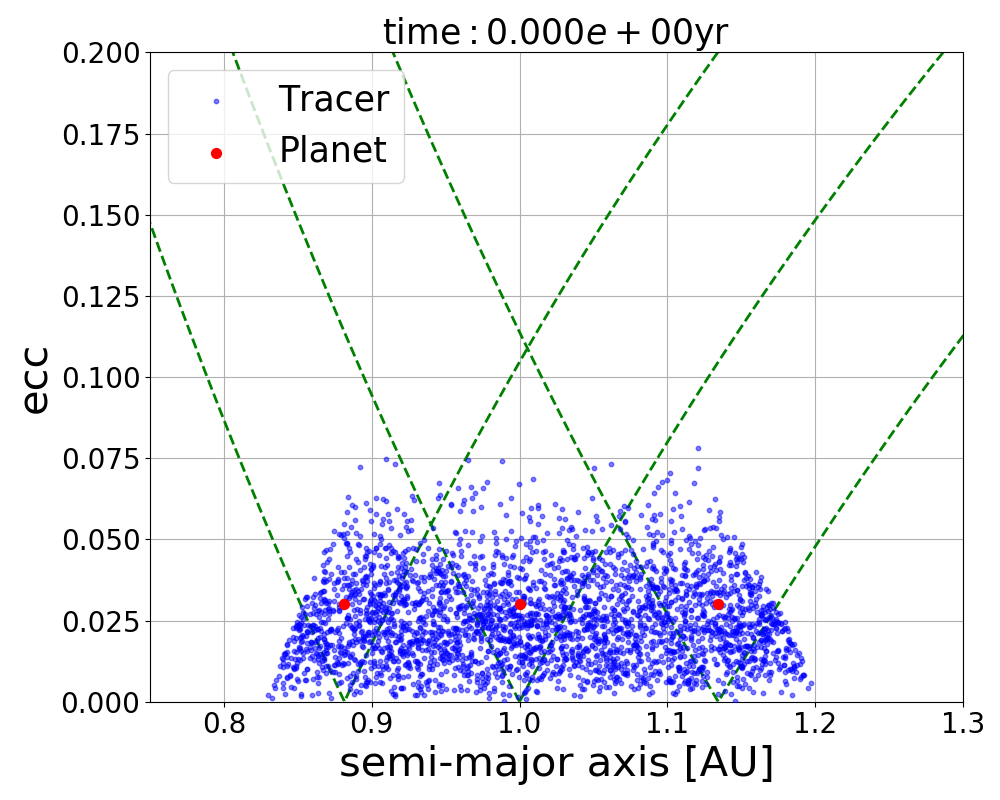
\includegraphics[width=\textwidth]{./image/axis_ecc_T00_nofrag_rand08.png}
\subcaption{初期}
\end{minipage} &
%右
\begin{minipage}[t]{0.5\hsize}
\centering
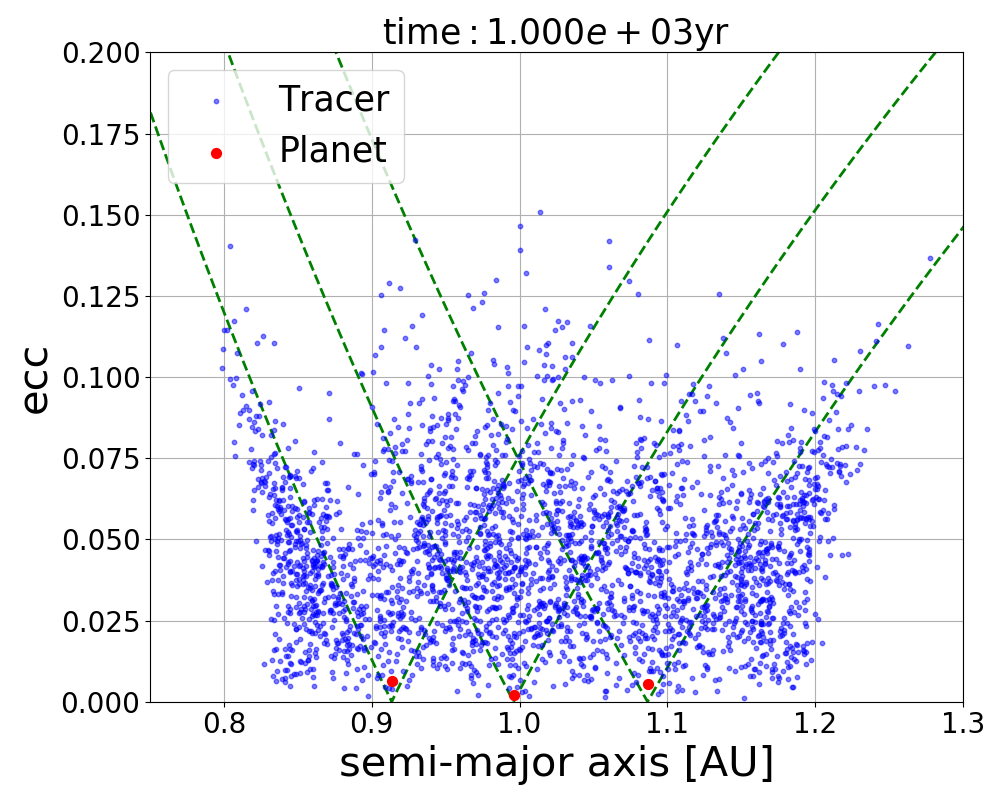
\includegraphics[width=\textwidth]{./image/axis_ecc_T33_nofrag_rand08.png}
\subcaption{破壊なし}
\end{minipage}\\
%
\end{tabular}\\
\begin{tabular}{cc}
%左
\begin{minipage}[t]{0.5\hsize}
\centering
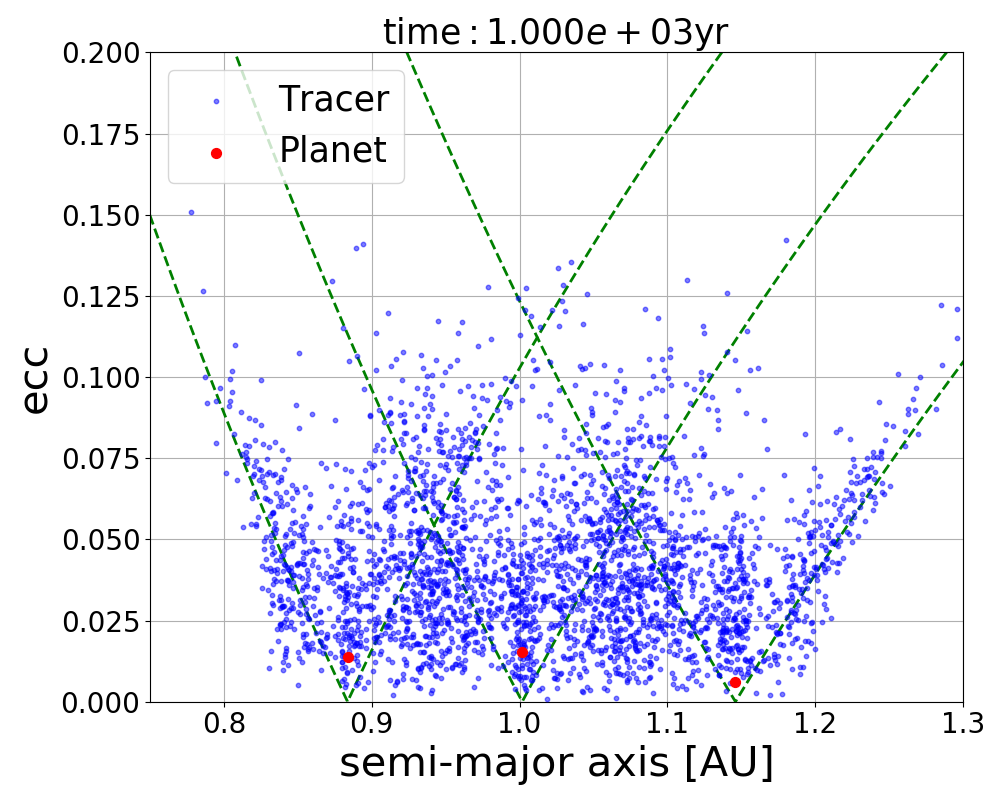
\includegraphics[width=\textwidth]{./image/axis_ecc_T33_frag_1E19_rand08.png}
\subcaption{破壊あり$m_{\rm max}=10^{19} \rm g$}
\end{minipage} &
%右
\begin{minipage}[t]{0.5\hsize}
\centering
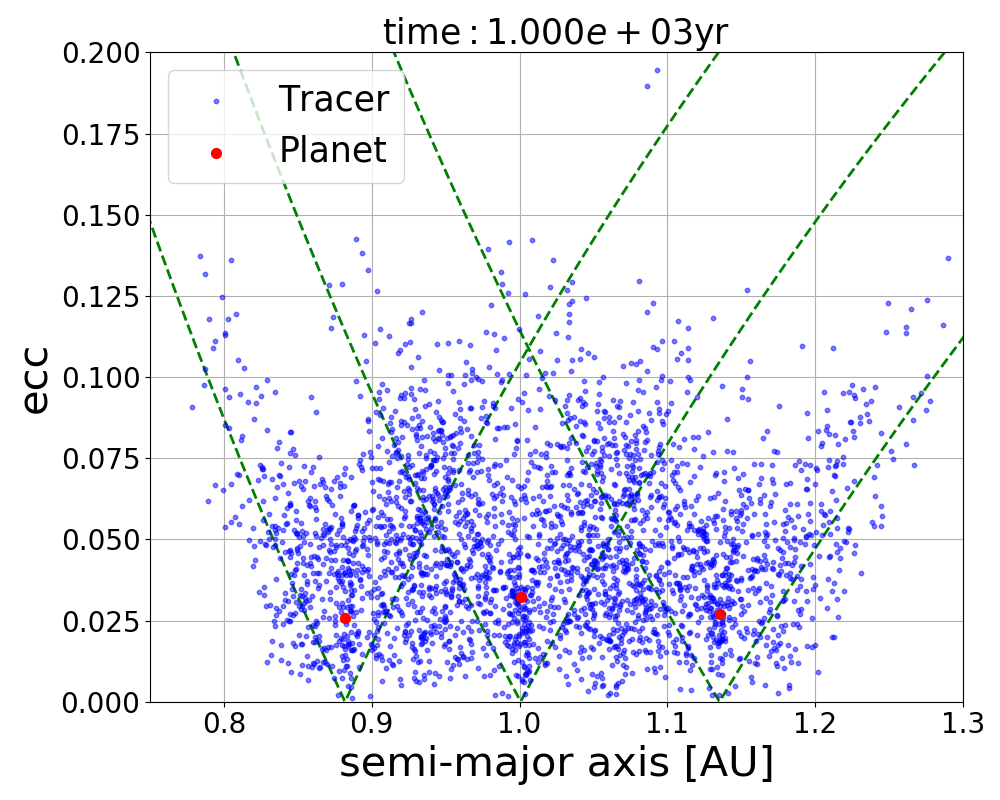
\includegraphics[width=\textwidth]{./image/axis_ecc_T33_frag_1E16_rand08.png}
\subcaption{破壊あり$m_{\rm max}=10^{16} \rm g$}
\end{minipage}\\
%
\end{tabular}
\caption{縦軸 : 離心率、横軸 : 軌道長半径としたときの惑星と微惑星の軌道の様子。赤点は惑星、青点は微惑星を代表させたトレーサー、緑破線は等ヤコビエネルギー線に対応している。(a)初期の軌道。(b)破壊を考慮しない場合の1000年後の軌道。(c)破壊を考慮し最大微惑星の質量を$10^{19} \rm g$にした場合の1000年後の軌道。(d)破壊を考慮し最大微惑星の質量を$10^{16} \rm g$にした場合の1000年後の軌道。\label{fig:axis_ecc3}}
\end{figure}


巨大衝突ステージにおいて、地球型惑星と残存微惑星との力学的摩擦を模擬したテスト計算を行い、微惑星同士の破壊を考慮する場合としない場合の比較を行った。
初期条件は、中心星($M_{\odot}$)から$1 {\rm AU}$の位置に3つの惑星($e_{\rm p}=0.03, i_{\rm p}=0.015, m_{\rm p}=1{\rm M_{\oplus}}$)を10相互ヒル半径の間隔で配置し、また$1 {\rm AU} \pm$ 15相互ヒル半径の位置に離心率と軌道傾斜角がレイリー分布の残存微惑星($e_{\rm rms}=0.03, i_{\rm rms}=0.015, m_{\rm tot}=10{\rm M_{\oplus}}$)を3000個のトレーサーで代表させ配置した。
ここで、天体$i$と隣の天体$i+1$の相互ヒル半径は$R_{\rm H,M}=(a_i + a_{i+1})/2~((m_i + m_{i+1})/3M_{\ast})^{1/3}$のように定義される。
破壊を考慮しない場合、破壊を考慮し最大微惑星の質量を$10^{19} {\rm g},10^{16} {\rm g}$にした場合の計3種類を1000年分計算したところ、図~\ref{fig:axis_ecc3},~\ref{fig:ecc3_sigma},~\ref{fig:ecc3_time}のようになった。
ここで3種類の計算について初期角度を変えた計算をそれぞれ13runずつ行っており、図~\ref{fig:ecc3_sigma}ではデータ点 : 平均値、エラーバー : 標準偏差とし、図~\ref{fig:ecc3_time}ではデータ点 : 2乗平均平方根、エラーバー : 標準偏差としている。


\begin{figure}[t]
 \centering
 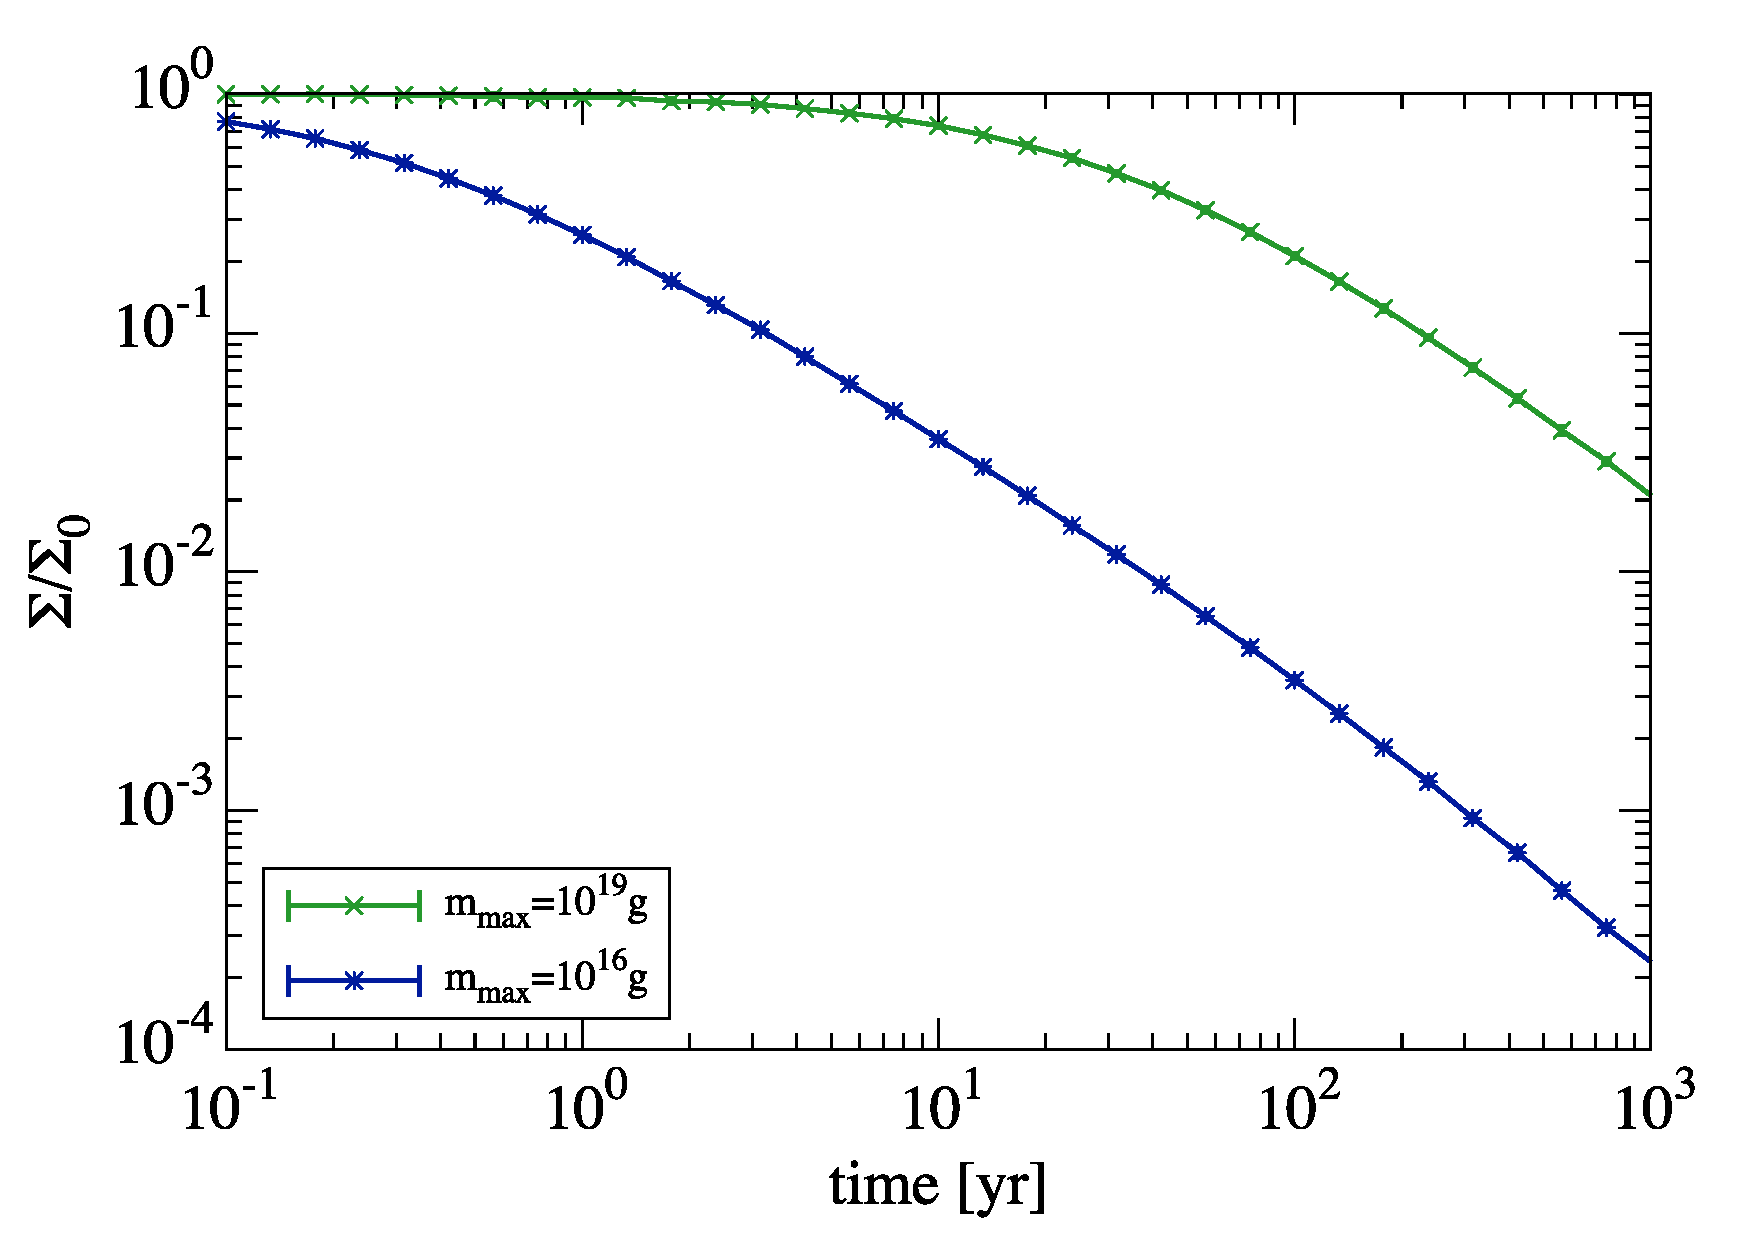
\includegraphics[width=8cm]{./image/Ntr3E3_t1E3_dtlog_Mtot3E-5_ecc3E-2_frag_Sigma_1E19_1E16.pdf}
 \caption{縦軸 : 初期面密度で規格化した面密度、横軸 : 時間としたときの面密度進化の様子。緑線と青線は最大微惑星の質量をそれぞれ$10^{19} {\rm g},10^{16} {\rm g}$にした場合に対応している。\label{fig:ecc3_sigma}}
\end{figure}

\begin{figure}[t]
 \centering
 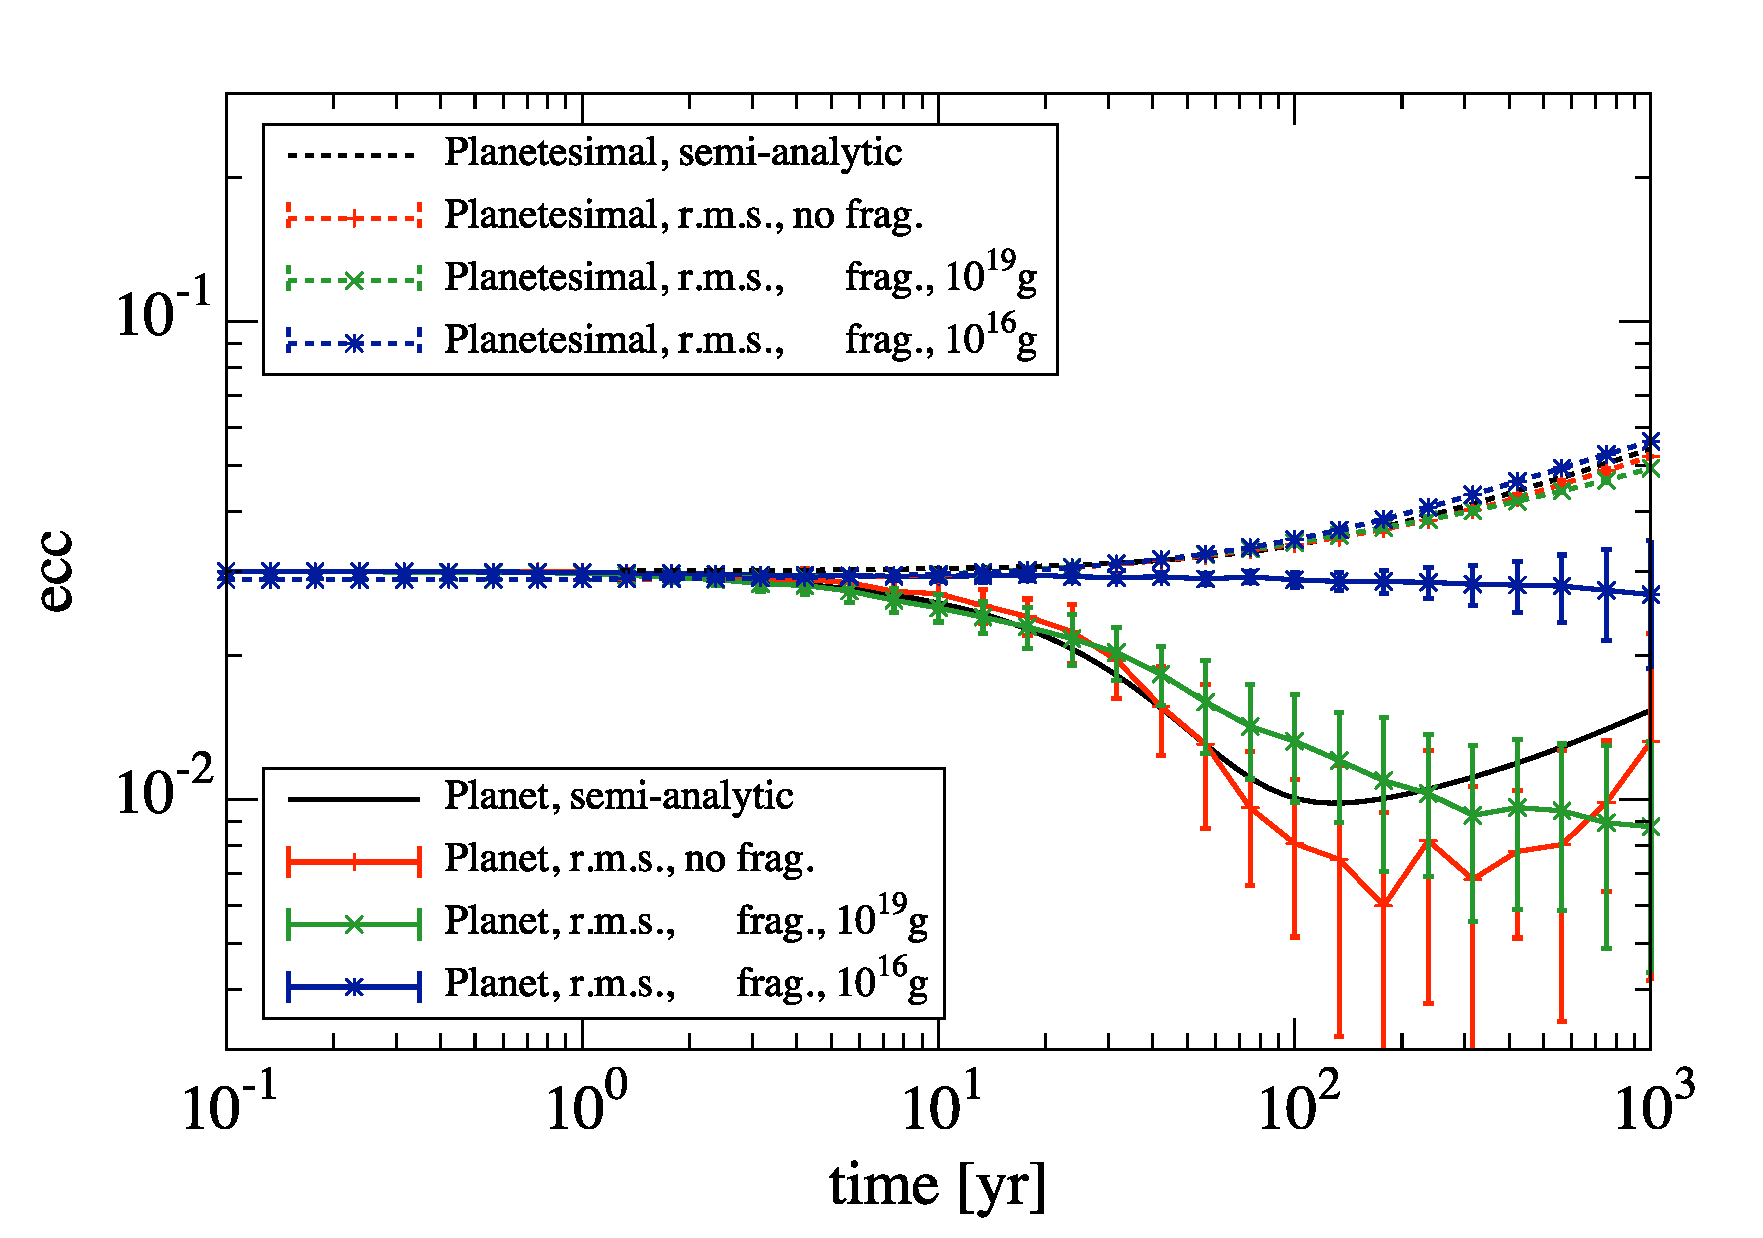
\includegraphics[width=8cm]{./image/Ntr3E3_t1E3_dtlog_Mtot3E-5_ecc3E-2_noacc_ecc_wf_wof.pdf}
 \caption{縦軸 : 離心率、横軸 : 時間としたときの離心率進化の様子。実線は惑星、破線は微惑星を代表させたトレーサーに対応している。また赤色は破壊を考慮しない場合、緑色と青色は破壊を考慮し最大微惑星の質量をそれぞれ$10^{19} {\rm g},~10^{16} {\rm g}$にした場合、黒色は平均離心率の変化率の解析解\citep[e.g.,][]{Ohtsuki_etal_2002}を数値積分したものに対応している。\label{fig:ecc3_time}}
\end{figure}

これらの結果は、破壊のタイムスケール$\tau_{\rm dep}$と力学的摩擦のタイムスケール$\tau_{\rm df}$を比較することで惑星の離心率の下がり方を説明できる。
$m_{\rm max}=10^{16} \rm g$は$\tau_{\rm dep} \ll \tau_{\rm df}$の場合であり、惑星の離心率はほとんど下がらなかった。
また$m_{\rm max}=10^{19} \rm g$は$\tau_{\rm dep} \lesssim \tau_{\rm df}$の場合であり、惑星の離心率の下がり方は緩やかではあるが力学的摩擦が効いている。
\par
このようなテスト計算の結果、巨大衝突ステージにおいて残存微惑星間の衝突・破壊現象を考慮すると、実際に惑星-微惑星間の力学的摩擦の効率が下がることを確かめることができた。







\section*{謝辞}

本研究を行うにあたり、様々なご指導を頂きました小林浩氏に深く感謝いたします。

\small
\bibliography{myref}
\bibliographystyle{apj}

\end{document}
